\documentclass[Report1]{subfiles}

\begin{document}
\section{Circuit Validation}
Two scripts were written to test the circuit. The first covered each of the simple cases:\\
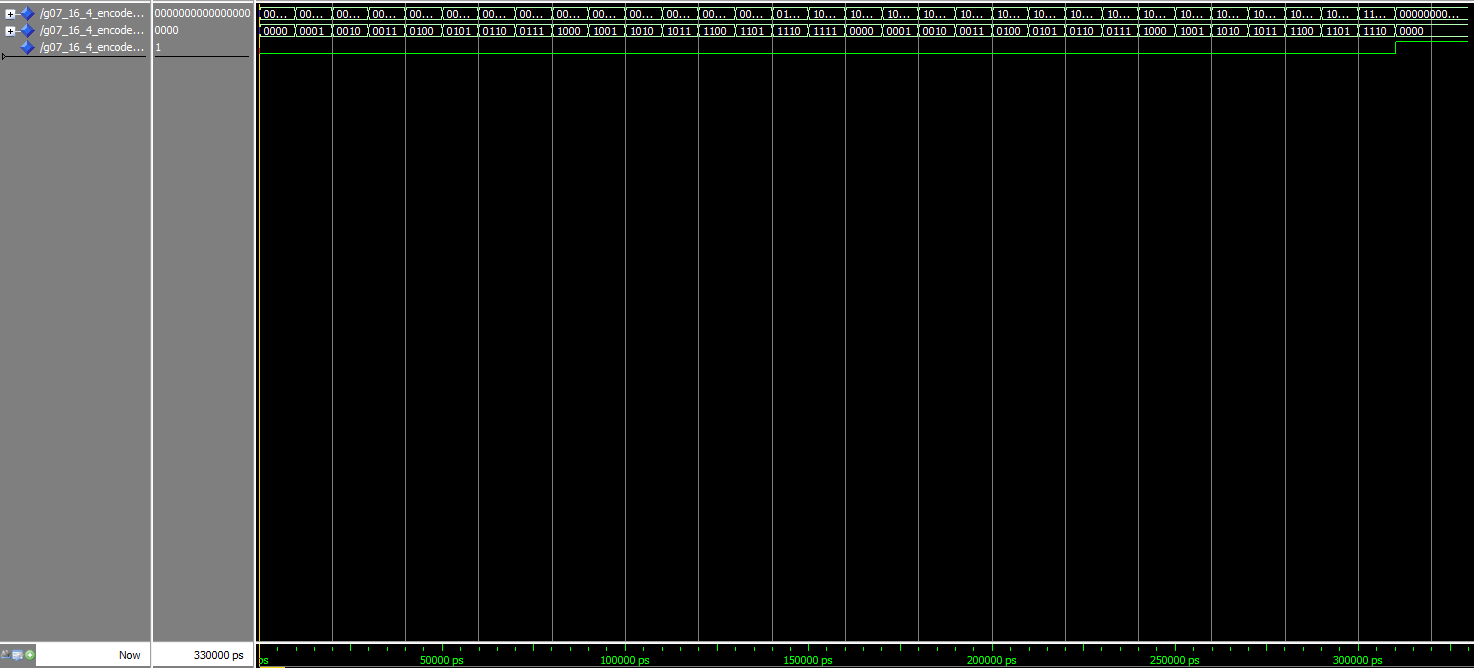
\includegraphics[width=\textwidth]{lab_1_full_16_test}
With a single high bit:\\
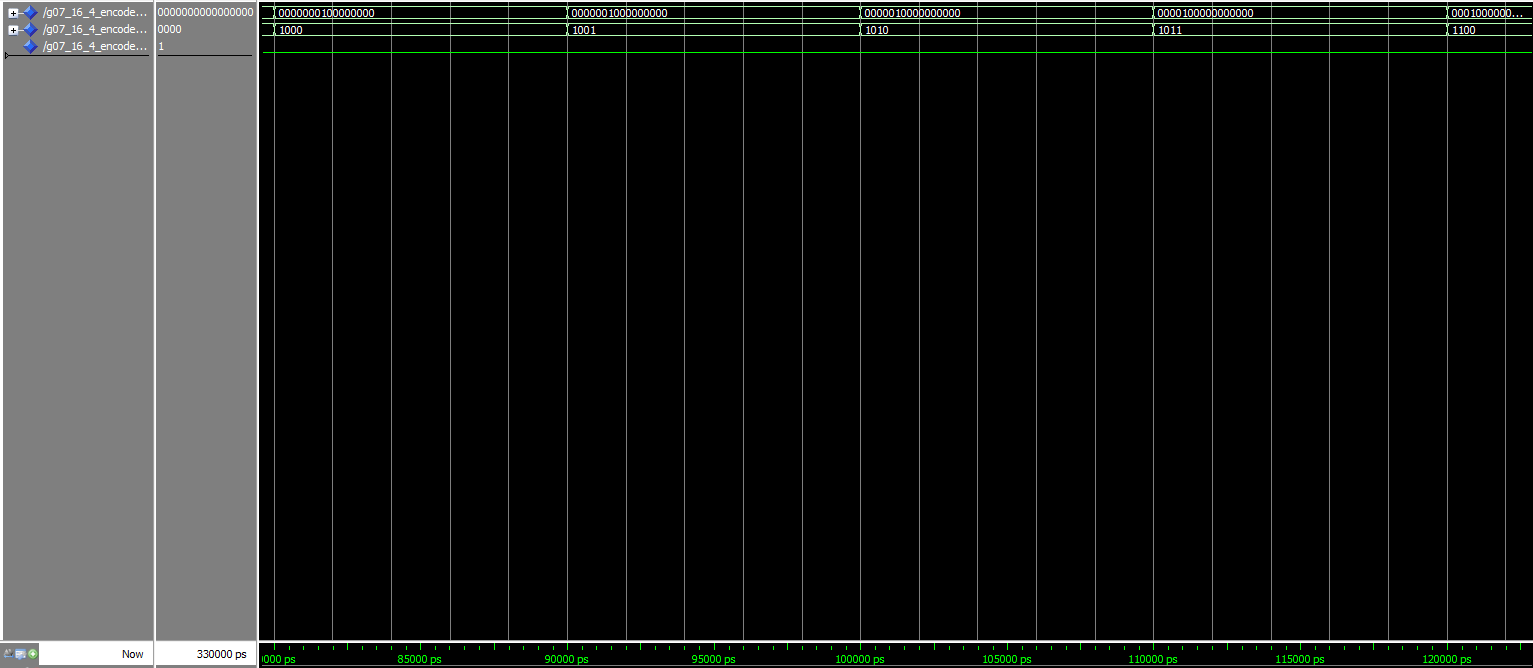
\includegraphics[width=\textwidth]{lab_1_simple_16_test}
The error case, where all bits were low, and then a set of more complex cases, where there were two high bits:\\
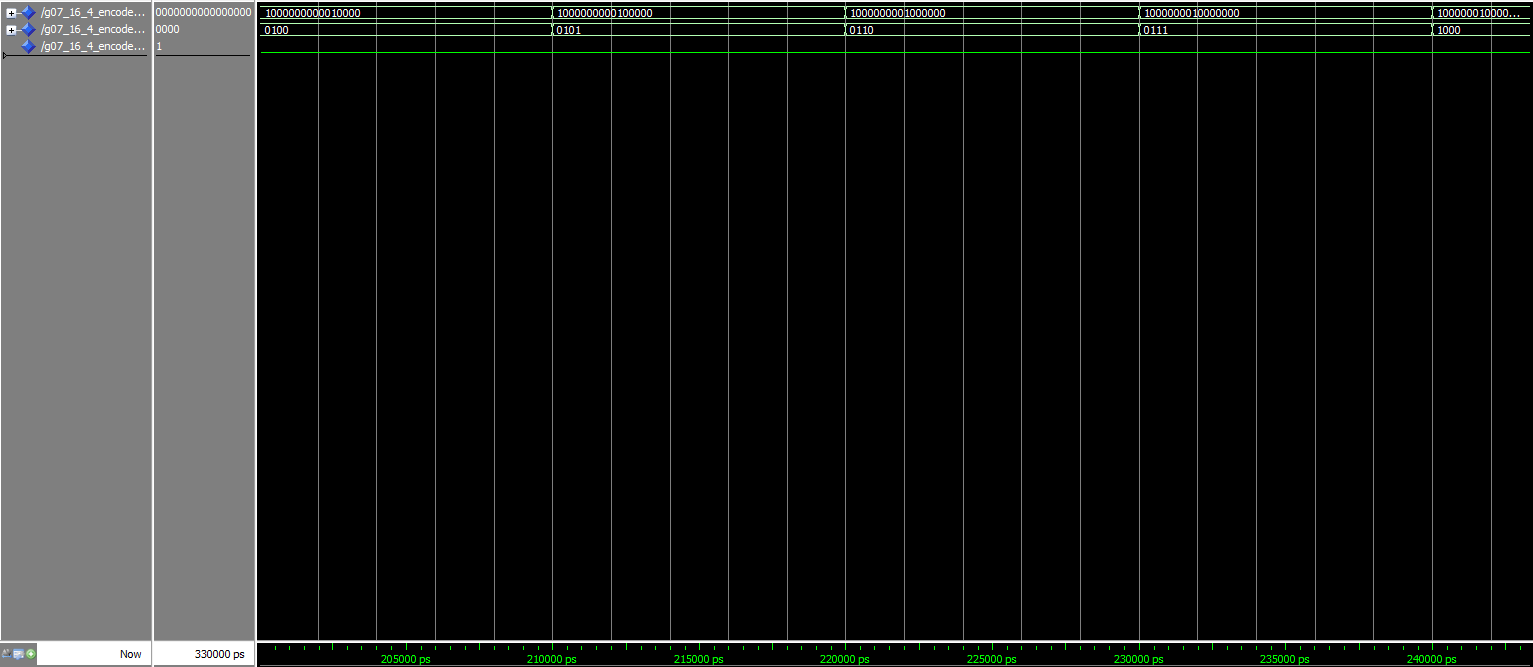
\includegraphics[width=\textwidth]{lab_1_multi_16_test}
Because the code for the circuit should function regardless of the number of extra high bits, testing with one extra was assumed to cover all such cases. \\
To double check, an exhaustive case was written, which generated all possible outputs. This was also run, and various points were inspected. Those were the cases from the limited test (to ensure matching results), other points, such as having all 1's except the 16th bit, and all 0's but the 16th bit, were checked to verify that the circuit was correctly handling the multiple-high cases. 
\end{document}